\documentclass[tikz,border=6pt]{standalone}
\usepackage{tikz}
\usetikzlibrary{arrows.meta,positioning}
\definecolor{navy}{HTML}{1E2B55}
\definecolor{blue}{HTML}{1769AA}
\definecolor{gold}{HTML}{B8860B}
\begin{document}
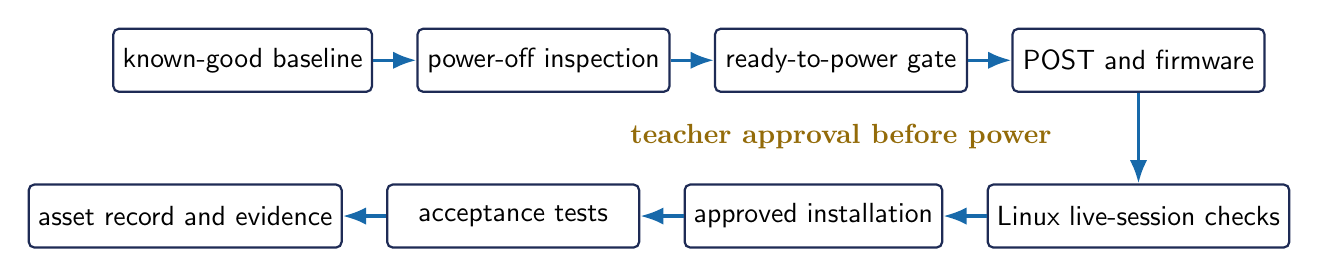
\begin{tikzpicture}[font=\sffamily,>=Latex,node distance=0.55cm]
  \tikzset{flowbox/.style={draw=navy,thick,rounded corners=2pt,minimum width=3.2cm,minimum height=0.8cm,align=center,fill=white}}
  \node[flowbox] (base) {known-good baseline};
  \node[flowbox,right=of base] (inspect) {power-off inspection};
  \node[flowbox,right=of inspect] (gate) {ready-to-power gate};
  \node[flowbox,right=of gate] (post) {POST and firmware};
  \node[flowbox,below=1.15cm of post] (live) {Linux live-session checks};
  \node[flowbox,left=of live] (install) {approved installation};
  \node[flowbox,left=of install] (accept) {acceptance tests};
  \node[flowbox,left=of accept] (record) {asset record and evidence};
  \draw[blue,very thick,->] (base) -- (inspect);
  \draw[blue,very thick,->] (inspect) -- (gate);
  \draw[blue,very thick,->] (gate) -- (post);
  \draw[blue,very thick,->] (post) -- (live);
  \draw[blue,very thick,->] (live) -- (install);
  \draw[blue,very thick,->] (install) -- (accept);
  \draw[blue,very thick,->] (accept) -- (record);
  \node[text=gold!80!black,font=\bfseries,below=0.28cm of gate] {teacher approval before power};
\end{tikzpicture}
\end{document}
